% !TEX root = ../main.tex
% 本文件由 build-tex.sh 从 11-DSP指南-第11章中译.md 生成，改内容请改 md 后重新生成

\chapter{傅里叶变换对}\label{ch-11}

每个时域波形都有一个对应的频域波形，反过来也一样。例如，时域中的矩形脉冲(rectangular
pulse)对应频域中的 sinc 函数（即
sin(x)/x）。对偶性(duality)保证反过来也成立：频域中的矩形脉冲对应时域中的
sinc 函数。像这样彼此对应的波形叫做傅里叶变换对(Fourier transform
pair)。本章介绍几种常见的变换对。

\section{冲激函数变换对}

对离散信号来说，冲激函数(delta
function)是一个简单的波形，它的傅里叶变换对也同样简单。图 11-1a
是时域中的一个冲激函数，(b) 和 (c)
是它的频谱。幅度(magnitude)是一个常数，相位(phase)则处处为零。上一章讲过，这可以用扩展/压缩性质(expansion/compression
property)来理解：时域被压缩到变成一个冲激时，频域就被扩展到变成一个常数。

在 (d) 和 (g) 中，时域波形分别向右平移了 4 个和 8
个采样。正如上一章的性质所预期的，时域波形的平移不影响幅度，但给相位加上了一个线性分量。本图中的相位信号没有展开(unwrapped)，所以只在
−π 到 π 之间。还要注意，频域的横轴从 −0.5 到
0.5，也就是说，图中除了正频率还画出了频谱的负频率(negative
frequencies)。负频率是冗余信息，但 DSP
的图里经常会画上它们，你应该习惯看到它们。

\begin{figure}[htbp]
\centering
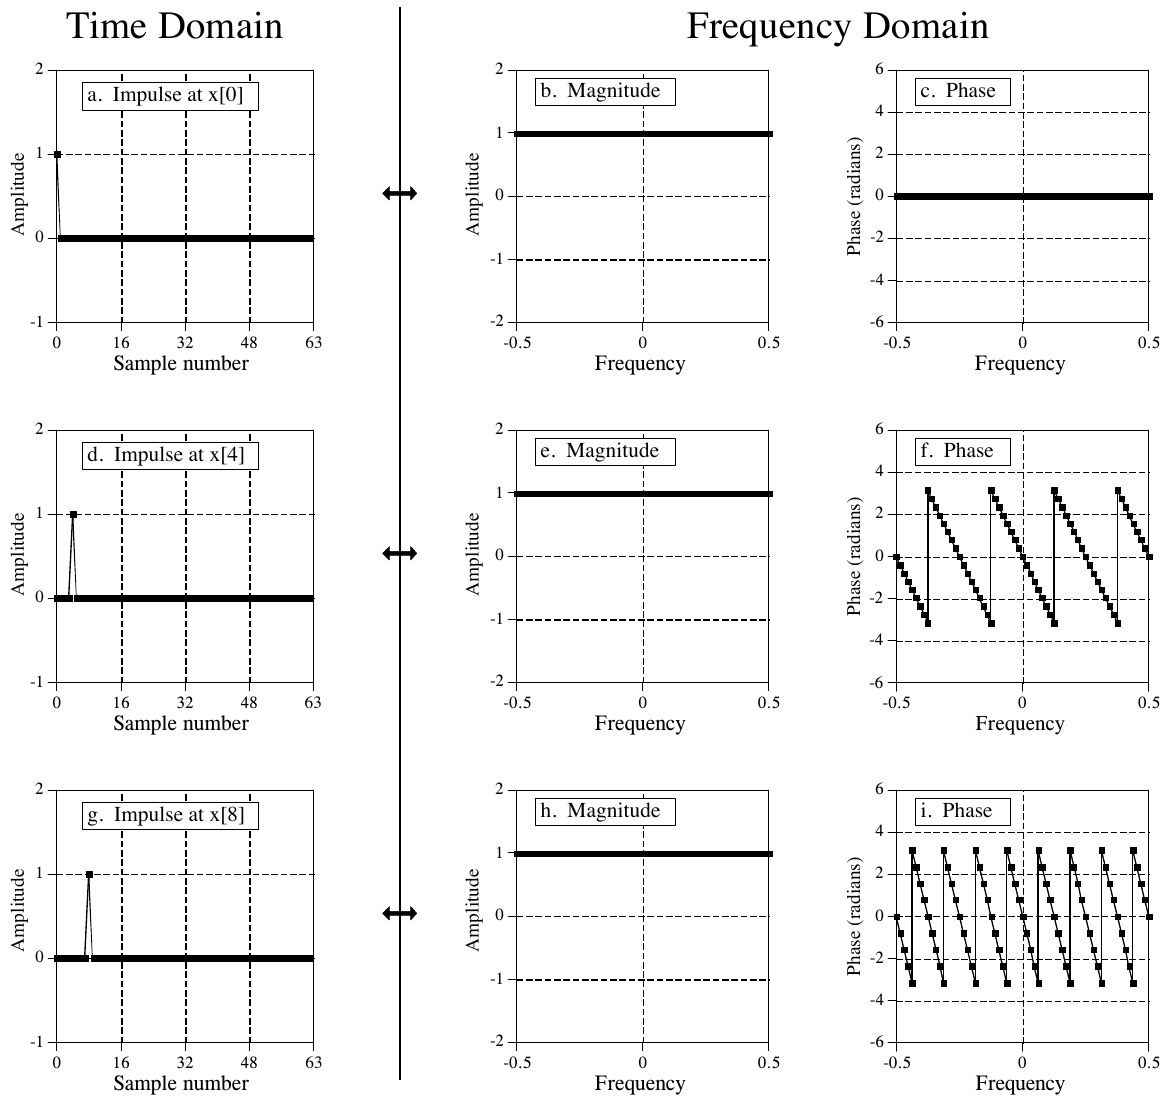
\includegraphics[width=0.975\linewidth,height=0.8\textheight,keepaspectratio]{assets/ch11/fig11-01.png}
\caption*{\textbf{图 11-1　极坐标形式的冲激函数变换对。}
时域中的一个冲激，对应频域中的常数幅度和线性相位。 （Time Domain =
时域，Frequency Domain = 频域；a. Impulse at x{[}0{]} = 位于 x{[}0{]}
的冲激，b. Magnitude = 幅度，c.~Phase = 相位；d、g 分别是位于
x{[}4{]}、x{[}8{]} 的冲激，e、h 为幅度，f、i 为相位。Amplitude =
幅度，Phase (radians) = 相位（弧度），Sample number =
采样序号，Frequency = 频率；中间的 \dspsym{↔} 表示左右两边互为变换对。）}
\end{figure}

图 11-2 给出了与图 11-1 相同的信息，只是频域改用直角坐标形式(rectangular
form)表示。这里有两点值得学习。第一，比较频域的极坐标表示和直角坐标表示。和通常一样，极坐标形式要好理解得多：幅度只是一个常数，相位是一条直线。相比之下，实部和虚部是正弦振荡，很难说出它们代表什么意思。

\begin{figure}[htbp]
\centering
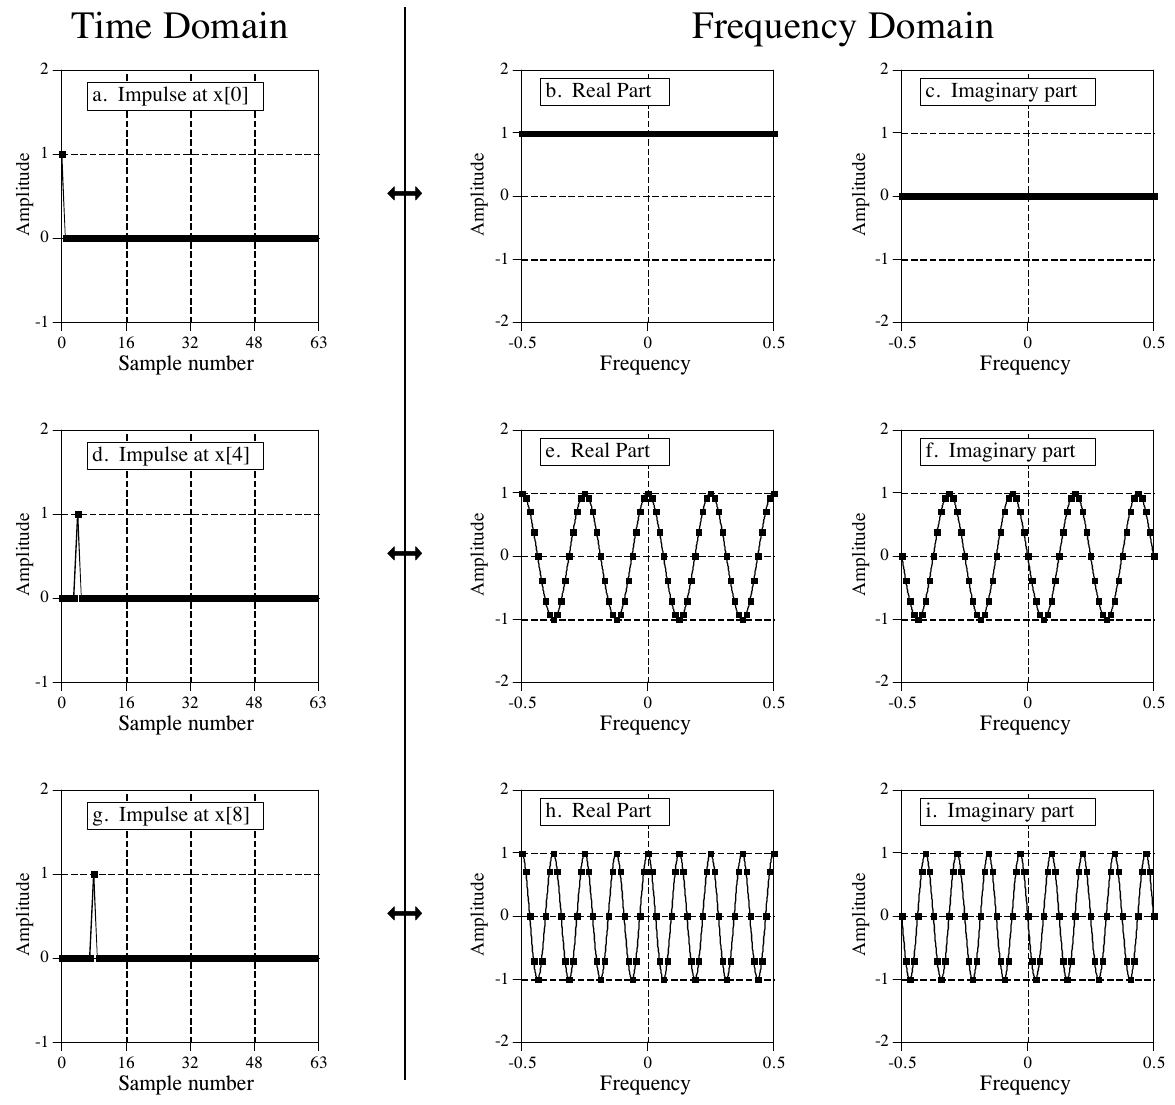
\includegraphics[width=0.979\linewidth,height=0.8\textheight,keepaspectratio]{assets/ch11/fig11-02.png}
\caption*{\textbf{图 11-2　直角坐标形式的冲激函数变换对。}
时域中的每个采样，在频域的实部产生一个余弦波，在虚部产生一个负的正弦波。
（Time Domain = 时域，Frequency Domain = 频域；a、d、g. Impulse at
x{[}0{]}/x{[}4{]}/x{[}8{]} = 位于 x{[}0{]}/x{[}4{]}/x{[}8{]}
的冲激；b、e、h. Real Part = 实部；c、f、i. Imaginary part =
虚部。Amplitude = 幅度，Sample number = 采样序号，Frequency = 频率。）}
\end{figure}

图 11-2 的第二个有趣之处是 DFT 的对偶性。按通常的看法，DFT
频域中的每个采样对应时域中的一个正弦信号(sinusoid)。然而反过来也成立：时域中的每个采样对应频域中的正弦信号。在图中画出负频率，能让对偶性显得更对称。例如，图
(d)、(e)、(f) 表明，时域中第 4 个采样处的一个冲激，在频谱的实部产生 4
个周期的余弦波，在虚部产生 4 个周期的负正弦波。回想一下，频谱实部第 4
个采样处的冲激，在时域产生 4 个周期的余弦波；同样，频谱虚部第 4
个采样处的冲激，会在时域波形上叠加 4 个周期的负正弦波。

第 8 章提到过，这可以用作计算 DFT
的另一种方法（除了把时域信号与正弦信号做相关之外）。时域中的每个采样，都会在频域实部加上一个余弦波，在虚部加上一个负正弦波。每个正弦信号的幅度由该时域采样的幅度给出，频率由该时域点的采样序号给出。算法步骤是：(1)
逐个遍历时域采样；(2) 算出每个采样对应的正弦波和余弦波；(3)
把所有贡献的正弦信号加起来。得到的程序和相关法（表
8-2）几乎一模一样，只是内外两层循环互换了。

\section{sinc 函数}

图 11-3 展示了一个常见的变换对：矩形脉冲与 sinc 函数(sinc function，读作
``sink'')。sinc 函数的定义是
\(\mathrm{sinc}(a) = \sin(\pi a)/(\pi a)\)，不过常见到一种含糊的说法：``sinc
函数的一般形式是 \(\sin(x)/x\)''。换句话说，sinc 是一个幅度按 1/x
衰减的正弦波。在 (a) 中，矩形脉冲以第 0
个采样为中心对称放置，脉冲的一半在图的右侧，另一半在左侧。由于时域的周期性，DFT
把它看作一个完整的脉冲。这个信号的 DFT 画在 (b) 和 (c)
中，展开后的版本画在 (d) 和 (e) 中。

\begin{quote}
\textbf{译注：} 原文此处写的是''图 11-4''，但图 11-4 是 x 与 sin(x)
的比较图，矩形脉冲与 sinc 函数的变换对画在图 11-3 中，这里按图 11-3
翻译。
\end{quote}

先看展开后的频谱 (d) 和
(e)。展开后的幅度是一个随频率升高而幅度减小的振荡。相位全部为零，对一个关于第
0 个采样对称的时域信号来说，这正是应有的结果。我们用''展开幅度(unwrapped
magnitude)``这个说法，表示它可以取正值也可以取负值。按定义，幅度必须始终为正。(b)
和 (c) 就是这样处理的：在 (d) 中展开幅度为负的所有频率上，引入 π
的相移，使幅度全部变为正值。

在 (f) 中，信号经过平移，显示为一个连续的脉冲，但不再以第 0
个采样为中心。这不改变频域的幅度，但给相位加上了一个线性分量，使相位变得一团乱。那么用实部和虚部表示的频谱是什么样子呢？乱到根本不值得去操心。

一个 N 点时域信号，若其中包含一个宽 M 点、幅度为 1 的矩形脉冲，它的 DFT
频谱为：

\textbf{公式 11-1}　矩形脉冲的 DFT 频谱。式中 N
是时域信号的点数，其中除了相邻的 M 个点值为 1 之外，其余点全为
0。频谱存放在 X{[}k{]} 中，k 从 0 到 N/2。为避免除以零，取 X{[}0{]} =
M。正弦函数用弧度而不是角度。这个公式已经把信号的混叠考虑在内。

\[\mathrm{Mag}\;X[k] = \left|\,\frac{\sin(\pi k M / N)}{\sin(\pi k / N)}\,\right|\]

\begin{figure}[htbp]
\centering
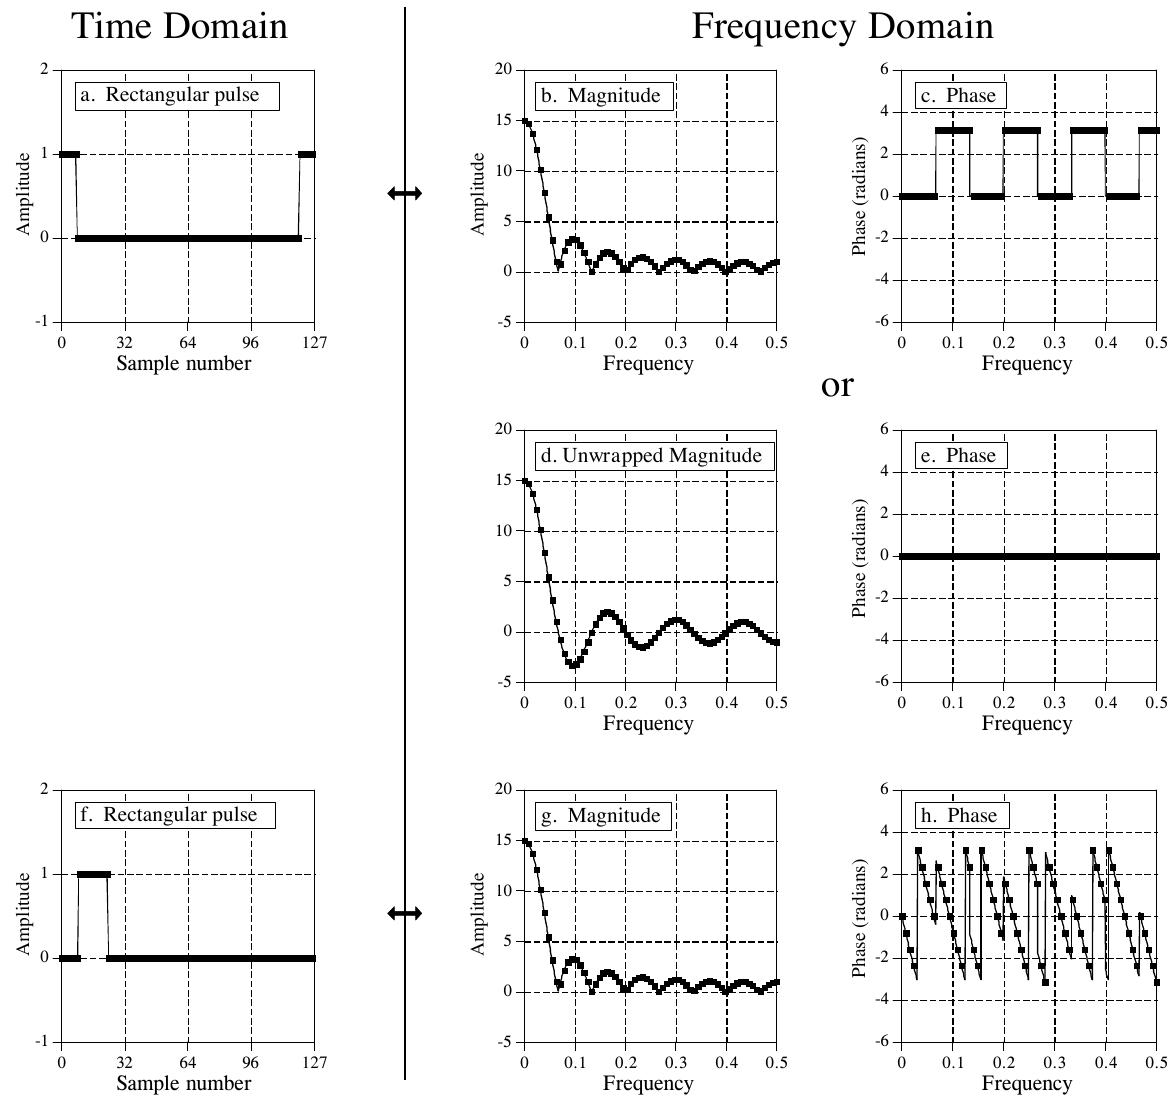
\includegraphics[width=0.979\linewidth,height=0.8\textheight,keepaspectratio]{assets/ch11/fig11-03.png}
\caption*{\textbf{图 11-3　矩形脉冲的 DFT。} 一个域中的矩形脉冲，对应另一个域中的
sinc 函数。 （Time Domain = 时域，Frequency Domain =
频域；a、f.~Rectangular pulse = 矩形脉冲；b、g. Magnitude =
幅度；c、e、h. Phase = 相位；d.~Unwrapped Magnitude = 展开幅度；中间的
or = 或者，表示 (b)(c) 与 (d)(e) 是同一频谱的两种表示。Amplitude =
幅度，Phase (radians) = 相位（弧度），Sample number =
采样序号，Frequency = 频率。）}
\end{figure}

另外，也可以用 DTFT 把频谱表示成采样率的分数 f 的函数：

\textbf{公式 11-2}　用采样频率改写的公式 11-1。参数 f 是采样率的分数，在
0 到 0.5 之间连续变化。为避免除以零，取 Mag X(0) = M。

\[\mathrm{Mag}\;X(f) = \left|\,\frac{\sin(\pi f M)}{\sin(\pi f)}\,\right|\]

（原书此公式的说明把 continuously 误拼成 continiously。）

换句话说，公式 11-1 给出频谱中的 N/2 + 1 个采样，而公式 11-2
给出这些采样所在的连续曲线。这两个公式只给出幅度。相位完全由时域波形的左右位置决定，上一章已经讨论过。

注意图 11-3b 中，振荡的幅度在频率到达 0.5
之前并没有衰减到零。你应该猜得到，这个波形会延续到下一个周期，在那里发生混叠(aliasing)。这改变了频域的形状，公式
11-1 和 11-2 已经把这种影响包括在内了。

了解没有混叠时频谱是什么样子，往往很重要。这是因为离散信号常常用来表示或模拟连续信号，而连续信号不会混叠。要去掉公式
11-1 和 11-2 中的混叠，只需把分母分别从 \(\sin(\pi k M/N)\) 改成
\(\pi k M/N\)、从 \(\sin(\pi f)\) 改成 \(\pi f\)。图 11-4
说明了这一改动的意义。由于 f 只能从 0 变到 0.5，πf 只能从 0 变到
1.5708。在这个范围内，\(\sin(\pi f)\) 和 \(\pi f\)
差别不大：在零频率处两者相等，在频率 0.5 处也只差约
36\%。如果没有混叠，图 11-3b
中的曲线在图的右侧会稍微低一点，在左侧则没有变化。

\begin{quote}
\textbf{译注：} 这里分母的写法照录原书。按公式 11-1、11-2
的形式，真正对应的分母是 \(\sin(\pi k/N)\) 和
\(\sin(\pi f)\)；原文第一处写成 \(\sin(\pi k M/N)\)（那是分子），应为
\(\sin(\pi k/N)\) 改成 \(\pi k/N\)。
\end{quote}

当矩形脉冲的频谱没有混叠时（因为时域信号是连续的，或者因为你忽略了混叠），它的一般形式是
\(\sin(x)/x\)，即 sinc 函数。对连续信号来说，矩形脉冲和 sinc
函数是傅里叶变换对；对离散信号来说这只是一种近似，误差来自混叠。

sinc 函数在 x = 0 处有一个恼人的问题：\(\sin(x)/x\)
变成了零除以零。这在数学上并不难办：当 x 变得非常小时，sin(x) 趋近于 x
的值（见图 11-4）。

\begin{figure}[htbp]
\centering
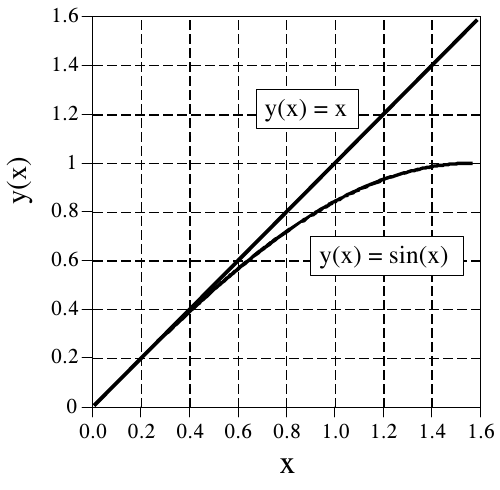
\includegraphics[width=0.417\linewidth,height=0.8\textheight,keepaspectratio]{assets/ch11/fig11-04.png}
\caption*{\textbf{图 11-4　x 与 sin(x) 的比较。} 函数 y(x) = x 和 y(x) = sin(x) 在
x 较小时很接近，在 1.57（π/2）处也只差约
36\%。这说明了混叠怎样使矩形脉冲的频谱偏离纯粹的 sinc 函数。
（图中两条曲线分别标注 y(x) = x 和 y(x) = sin(x)。）}
\end{figure}

这样 sinc 函数就变成了 x/x，其值为一。换句话说，当 x 越来越小时，sinc(x)
的值趋近于一，其中也包括 sinc(0) =
1。现在试着把这一点告诉你的计算机！它看到的只有除以零，于是会报错并让程序停下来。要记住的要点是：计算
sinc 函数时，程序必须对 x = 0 做特殊处理。

sinc
函数的一个关键特征是过零点的位置。它们出现在这样的频率上：正弦信号恰好有整数个周期能放进矩形脉冲里。例如，如果矩形脉冲宽
20 个点，频域中第一个零点位于''在 20
个点内完成一个完整周期''的频率处，第二个零点位于''在 20
个点内完成两个完整周期''的频率处，依此类推。回想 DFT
是怎样用相关计算的，就能理解这一点：一个频率分量的幅度，是把时域信号与一个正弦信号相乘、再把得到的采样加起来求得的。如果时域波形是一个幅度为
1
的矩形脉冲，这就等于把落在矩形脉冲内的那些正弦采样加起来。如果这个求和覆盖的是正弦信号的整数个周期，结果就是零。

sinc 函数在 DSP
中应用很广，因为它是一个非常简单的波形（矩形脉冲）的傅里叶变换对。例如，第
9 章讨论的频谱分析就用到了 sinc
函数。设想要分析一个无限长的离散信号。由于 DFT
只能处理有限长的信号，就选取 N
个采样来代表这个更长的信号。关键在于，``从长信号中选取 N
个采样''等同于把这个长信号乘以一个矩形脉冲：矩形脉冲中的 1
保留对应的采样，0
则把它们去掉。这对信号的频谱有什么影响呢？时域乘以一个矩形脉冲，导致频域与一个
sinc 函数卷积。这降低了频谱的分辨率，前面图 9-5a 已经展示过。

\section{其他变换对}

图 11-5 的 (a) 和 (b) 展示了上述内容的对偶：频域中的矩形脉冲对应时域中的
sinc 函数（加上混叠）。把混叠的影响包括在内，时域信号为：

\textbf{公式 11-3}　矩形脉冲的逆 DFT。在频域中，脉冲幅度为 1，从第 0
个采样一直到第 M−1 个采样。参数 N 是 DFT 的长度，x{[}i{]} 是时域信号，i
从 0 到 N−1。为避免除以零，取 x{[}0{]} = (2M−1)/N。

\[x[i] = \frac{1}{N}\,\frac{\sin\!\big(2\pi i\,(M - 1/2)/N\big)}{\sin(\pi i / N)}\]

要从这个公式中去掉混叠的影响，可以设想频域采样得无比精细，以至于变成一条连续曲线。这会使时域变成无限长、不再有周期性。这时该用的傅里叶变换是
DTFT，得到的时域信号由下面的关系给出：

\textbf{公式 11-4}　矩形脉冲的逆 DTFT。在频域中，脉冲幅度为
1，从零频率一直到截止频率 \(f_c\)，\(f_c\) 取 0 到 0.5
之间的值。时域信号存放在 x{[}i{]} 中，i 从 0 到 N−1。为避免除以零，取
x{[}0{]} = 2f\textsubscript{c}。

\[x[i] = \frac{\sin(2\pi f_c\, i)}{i\pi}\]

这个公式在 DSP
中非常重要，因为频域中的矩形脉冲就是理想的低通滤波器(perfect low-pass
filter)。因此，这个公式描述的 sinc
函数就是理想低通滤波器的滤波器核。这是一类非常有用的数字滤波器------加窗
sinc 滤波器(windowed-sinc filter)------的基础，第 15 章会介绍。

图 (c) 和 (d) 表明，时域中的三角形脉冲(triangular pulse)对应频域中的
sinc 平方（加上混叠）。这个变换对本身没有它成立的原因重要。一个 2M−1
点的三角形，可以由一个 M
点矩形脉冲与它自身卷积得到。由于时域卷积对应频域相乘，把一个波形与自身卷积，就会把它的频谱平方。

有没有一种波形，它的傅里叶变换就是它自己？答案是有，而且只有一种：高斯曲线(Gaussian)。图
(e) 是一条高斯曲线，(f)
是它对应的频谱，也是一条高斯曲线。只有忽略混叠时这个关系才成立。时域和频域标准差之间的关系为
\(2\pi\sigma_f = 1/\sigma_t\)。(f)
中只画出了高斯曲线的一侧，频谱中的负频率补全了整条曲线，对称中心在零频率处。

图 (g) 可以叫做高斯脉冲串(Gaussian
burst)。它由一个正弦波乘以一条高斯曲线构成。例如，(g) 就是一个正弦波乘以
(e)
中那条高斯曲线。对应的频域是一条中心不在零频率处的高斯曲线。和前面一样，这个变换对本身没有它成立的原因重要。由于时域信号是两个信号的乘积，频域就是这两个频谱的卷积。正弦波的频谱是位于该正弦波频率处的一个冲激函数；高斯曲线的频谱是以零频率为中心的一条高斯曲线。两者卷积，得到以正弦波频率为中心的一条高斯曲线。这应该看着眼熟：它和上一章介绍的调幅(amplitude
modulation)过程完全相同。

\begin{figure}[htbp]
\centering
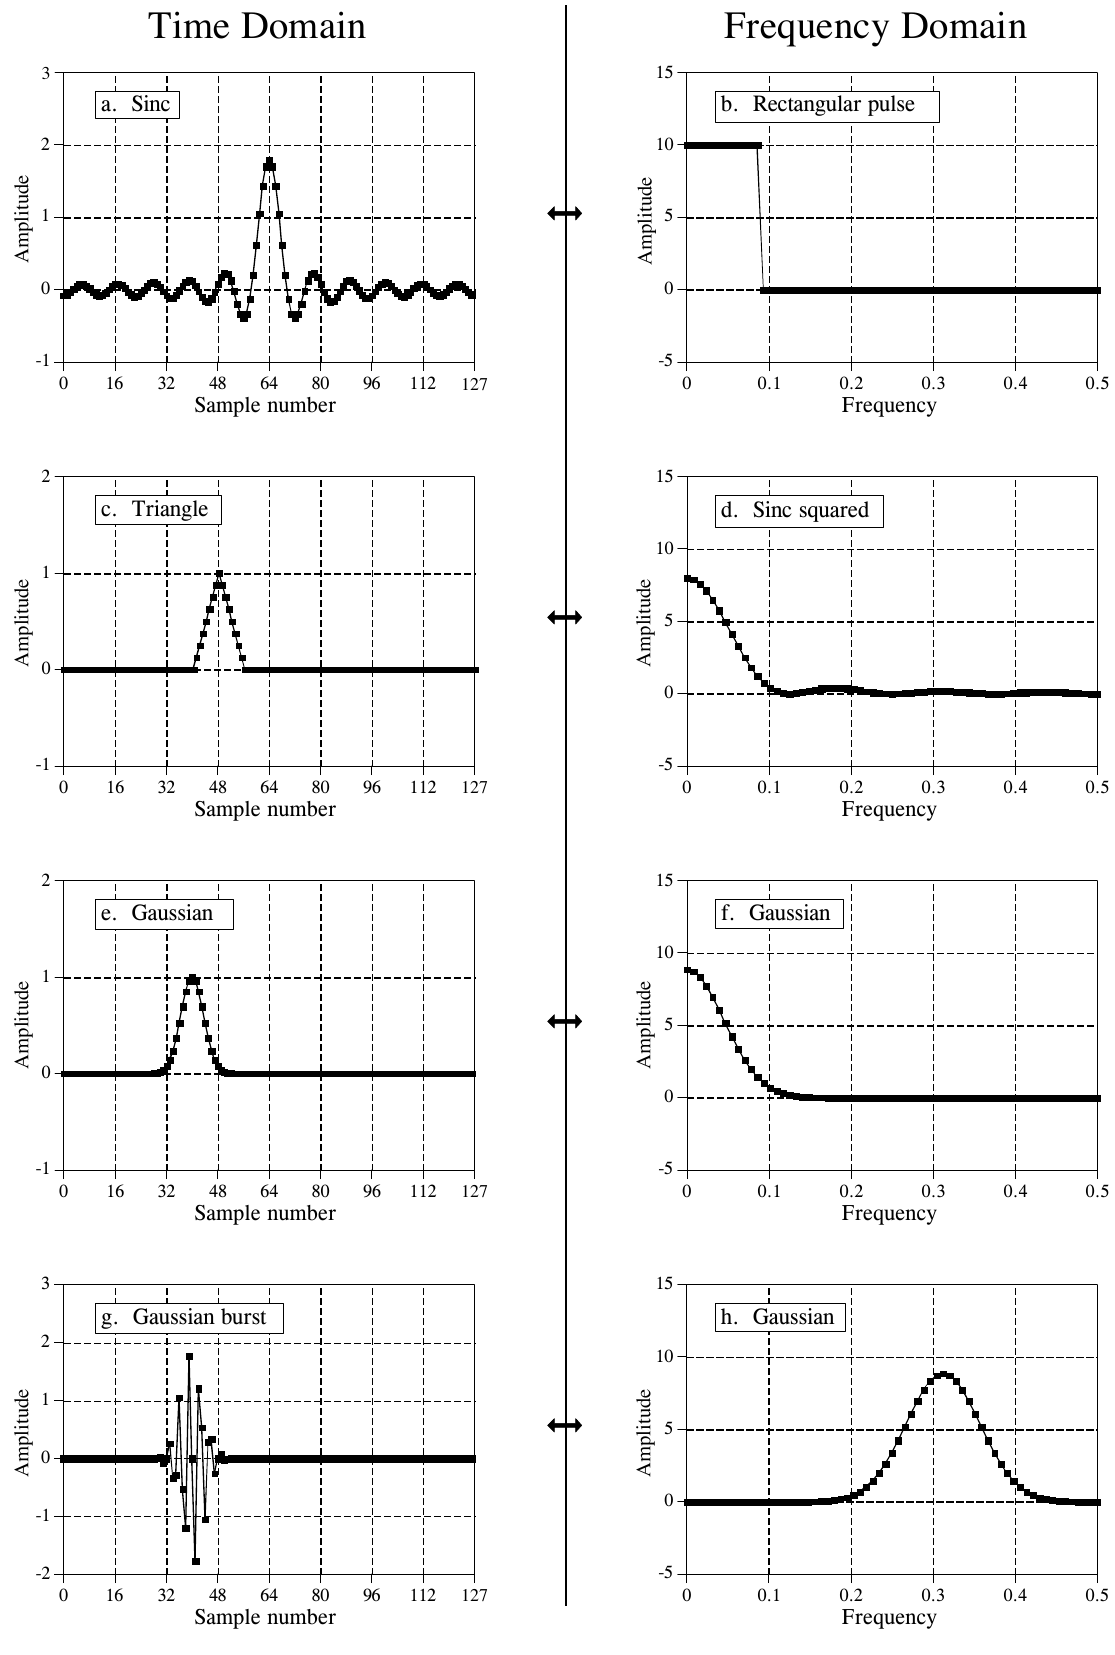
\includegraphics[width=0.929\linewidth,height=0.8\textheight,keepaspectratio]{assets/ch11/fig11-05.png}
\caption*{\textbf{图 11-5　常见的变换对。} （Time Domain = 时域，Frequency Domain
= 频域；a. Sinc = sinc 函数 \dspsym{↔} b. Rectangular pulse =
矩形脉冲；c.~Triangle = 三角形 \dspsym{↔} d.~Sinc squared = sinc
平方；e. Gaussian = 高斯曲线 \dspsym{↔} f.~Gaussian = 高斯曲线；g.
Gaussian burst = 高斯脉冲串 \dspsym{↔} h. Gaussian = 高斯曲线。Amplitude
= 幅度，Sample number = 采样序号，Frequency = 频率。）}
\end{figure}

\section{吉布斯效应}

图 11-6
展示了用正弦信号合成一个时域信号的过程。要重建的信号画在最后一幅图 (h)
中。这个信号长 1024 点，所以完整重建需要 513 个频率。图 (a) 到 (g)
展示了只用其中一部分频率时，重建出的信号是什么样子。例如，(f) 是用频率 0
到 100 重建的信号。它的做法是：对 (h) 中的信号做 DFT，把频率 101 到 512
设为零，再用逆 DFT 求出得到的时域信号。

重建中加入的频率越多，信号就越接近最终结果。有意思的是信号中的边沿处是怎样逼近最终结果的。(h)
中有三个陡峭的边沿：两个是矩形脉冲的边沿；第三个在第 1023 个采样和第 0
个采样之间，因为 DFT
把时域看作是周期性的。只用一部分频率重建时，每个边沿都会出现过冲(overshoot)和振铃（ringing，逐渐衰减的振荡）。这种过冲和振铃叫做吉布斯效应(Gibbs
effect)，以数学物理学家乔赛亚·吉布斯(Josiah Gibbs)的名字命名，他在 1899
年解释了这一现象。

仔细看 (e)、(f)、(g)
中的过冲。加入的正弦信号越多，过冲的宽度越窄；但过冲的幅度大致保持不变，约为
9\%。对离散信号来说这不成问题：加入最后一个频率时，过冲就消失了。然而，连续信号的重建就没那么好解释了。合成一个连续信号必须加入无穷多个正弦信号。问题在于，当正弦信号的个数趋于无穷时，过冲的幅度并不减小，而是保持在大约
9\%。鉴于这种情况（以及其他一些论点），人们有理由怀疑：连续正弦信号的求和到底能不能重建出一个边沿？还记得拉格朗日和傅里叶之间的那场争论吗？

解开这个谜题的关键在于：加入的正弦信号越多，过冲的宽度越小。正弦信号无穷多时过冲仍然存在，但宽度为零。恰好在间断点处，重建信号的值收敛到阶跃的中点。吉布斯证明，在''两者之间的误差能量为零''这个意义上，这个求和收敛到原信号。

与吉布斯效应有关的问题在 DSP
中经常遇到。例如，低通滤波器截掉了较高的频率，结果在时域的边沿处产生过冲和振铃。另一种常见的做法是截掉时域信号的两端，以免它们延伸到相邻的周期中去。根据对偶性，这会使频域中的边沿失真。这些问题会在后面讲滤波器设计的章节中再次出现。

\begin{figure}[htbp]
\centering
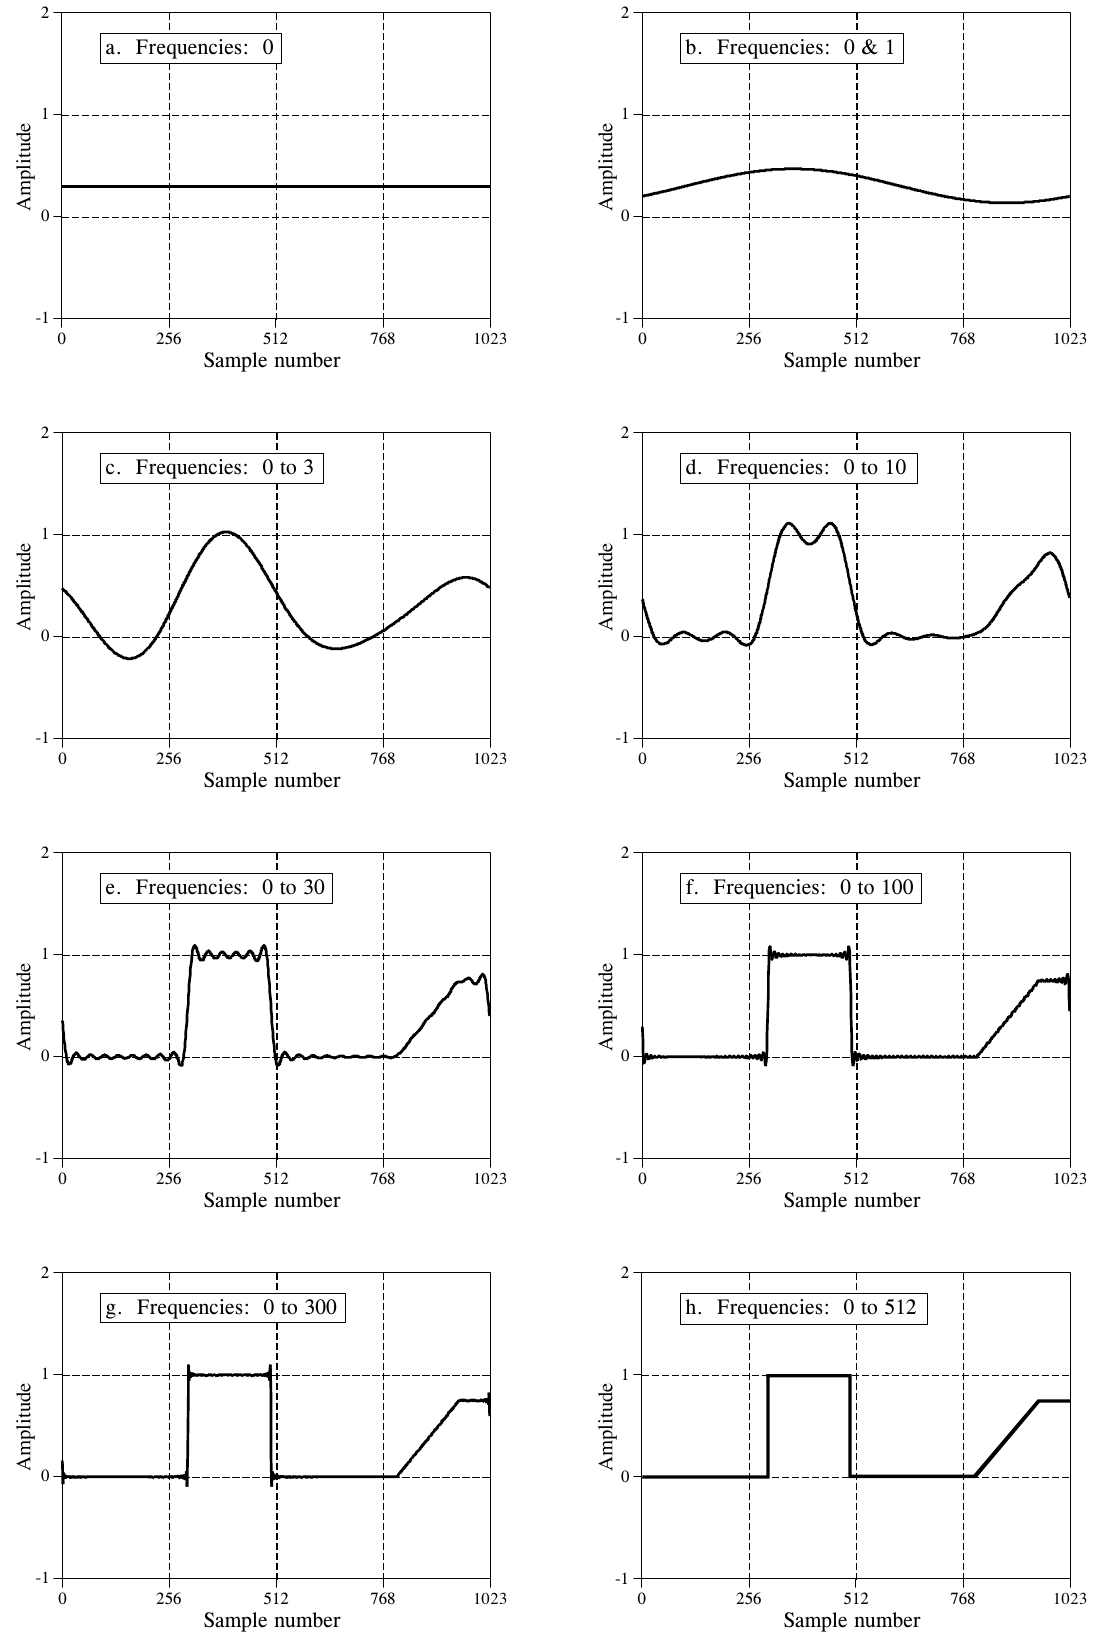
\includegraphics[width=0.917\linewidth,height=0.8\textheight,keepaspectratio]{assets/ch11/fig11-06.png}
\caption*{\textbf{图 11-6　吉布斯效应。} （a～h. Frequencies: 0 / 0 \& 1 / 0 to 3
/ 0 to 10 / 0 to 30 / 0 to 100 / 0 to 300 / 0 to 512 = 所用频率：0 / 0
和 1 / 0～3 / 0～10 / 0～30 / 0～100 / 0～300 / 0～512。Amplitude =
幅度，Sample number = 采样序号。）}
\end{figure}

\section{谐波}

如果一个信号以频率 f 呈周期性，那么组成这个信号的频率只有 f 的整数倍，即
f、2f、3f、4f 等。这些频率叫做谐波(harmonics)。一次谐波是 f，二次谐波是
2f，三次谐波是 3f，依此类推。一次谐波（即
f）还有一个专门的名字，叫基频(fundamental frequency)。图 11-7
是一个例子。图 (a) 是一个纯正弦波，(b) 是它的 DFT，只有一个峰。在 (c)
中，把正弦波的波峰顶部往里压，使正弦波发生失真。图 (d)
是这种失真在频域中的结果。由于失真后的信号仍以与原正弦波相同的频率呈周期性，频域由原来的峰加上若干谐波组成。谐波可以是任意幅度，不过通常随频率升高而变小。和任何信号一样，陡峭的边沿会带来更高的频率。例如，设想一个普通的
TTL 逻辑门产生 1 kHz 的方波。边沿在几纳秒内上升，会产生一直到将近 100
MHz 的谐波，也就是第一万次谐波！

\begin{figure}[htbp]
\centering
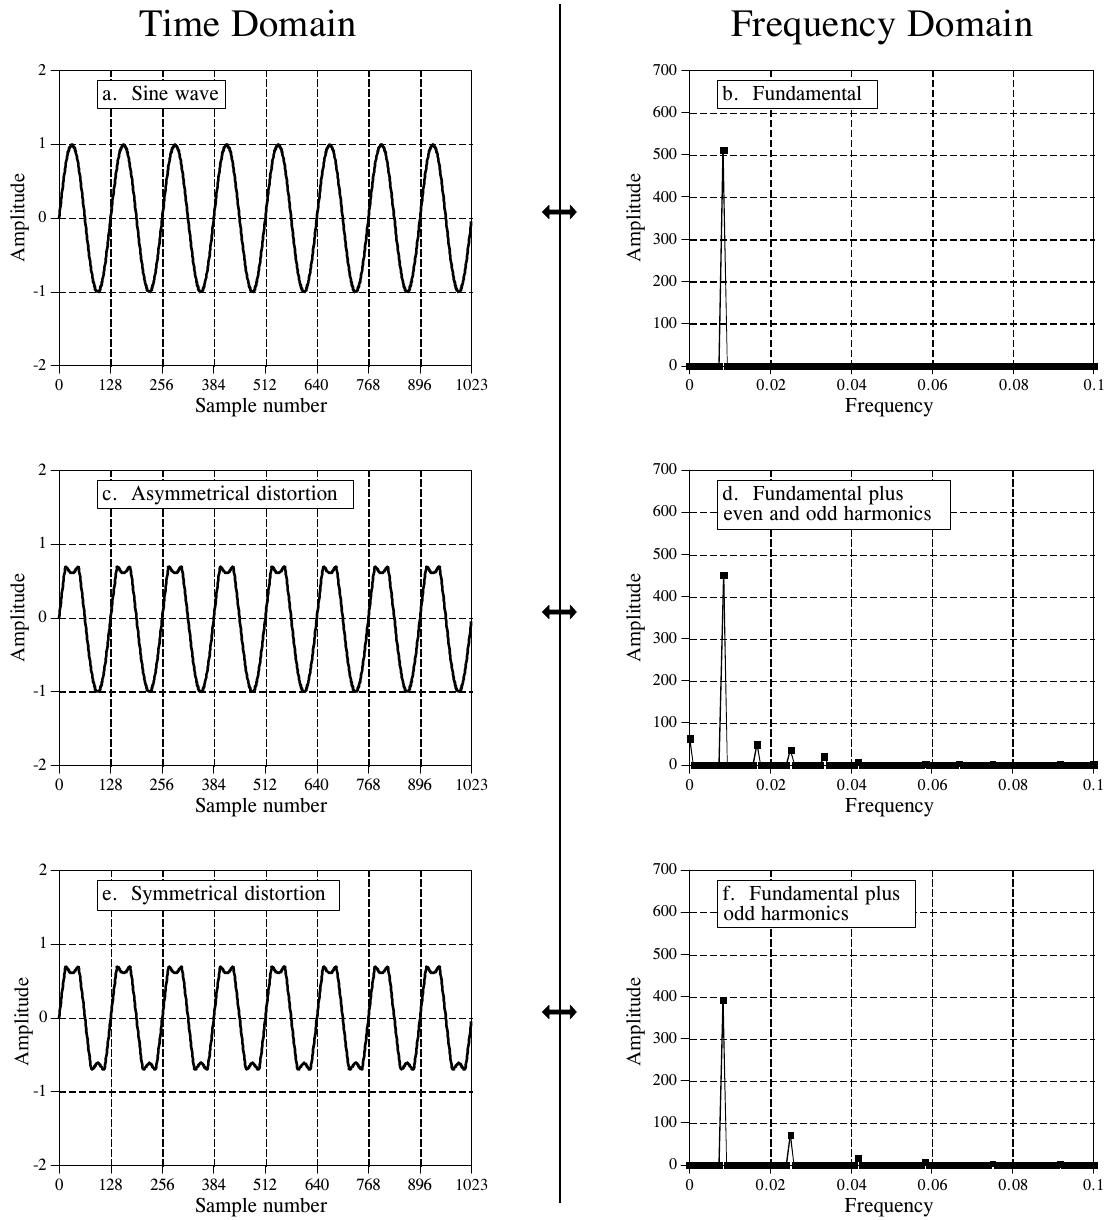
\includegraphics[width=0.925\linewidth,height=0.8\textheight,keepaspectratio]{assets/ch11/fig11-07.png}
\caption*{\textbf{图 11-7　谐波的例子。} (c) 中的不对称失真产生偶次和奇次谐波
(d)；而 (e) 中的对称失真只产生奇次谐波 (f)。 （Time Domain =
时域，Frequency Domain = 频域；a. Sine wave = 正弦波，b. Fundamental =
基波；c.~Asymmetrical distortion = 不对称失真，d.~Fundamental plus even
and odd harmonics = 基波加偶次和奇次谐波；e. Symmetrical distortion =
对称失真，f.~Fundamental plus odd harmonics = 基波加奇次谐波。Amplitude
= 幅度，Sample number = 采样序号，Frequency = 频率。）}
\end{figure}

\begin{quote}
\textbf{译注：} 原书图注写的是对称失真''只产生偶次谐波(only even
harmonics)``，与正文和图 (f)
的标注矛盾，应为''只产生奇次谐波''，这里按正确意思翻译。
\end{quote}

图 (e)
展示了谐波分析中的一个微妙之处。如果信号关于一条水平轴对称，即上半部分的波瓣是下半部分波瓣的镜像，那么所有偶次谐波的值都为零。如
(f) 所示，信号中只含有基波、三次谐波、五次谐波等。

所有连续的周期信号都可以像上面描述的那样，表示为谐波之和。离散的周期信号有一个问题，打乱了这种简单的关系。你大概已经猜到了，这个问题就是混叠。图
11-8a
是一个用同样方式（把波峰顶部往里压）失真了的正弦波。这个波形看起来远不如前一个例子那样规整平滑，因为这个正弦波的频率高得多，每个周期的采样点更少。图
(b)
是这个信号的频谱。不出所料，你能认出基波和谐波。这个例子表明，谐波可以延伸到高于采样频率
0.5 倍的频率上，并会混叠到 0 和 0.5 之间的某个频率。你在 (b)
中注意不到它们，因为它们的幅度太低。图 (c)
用对数刻度画出频谱，显示出这些低幅度的混叠峰。乍一看，这个频谱像随机噪声。其实不是，这是许多谐波混叠后相互重叠的结果。

\begin{figure}[htbp]
\centering
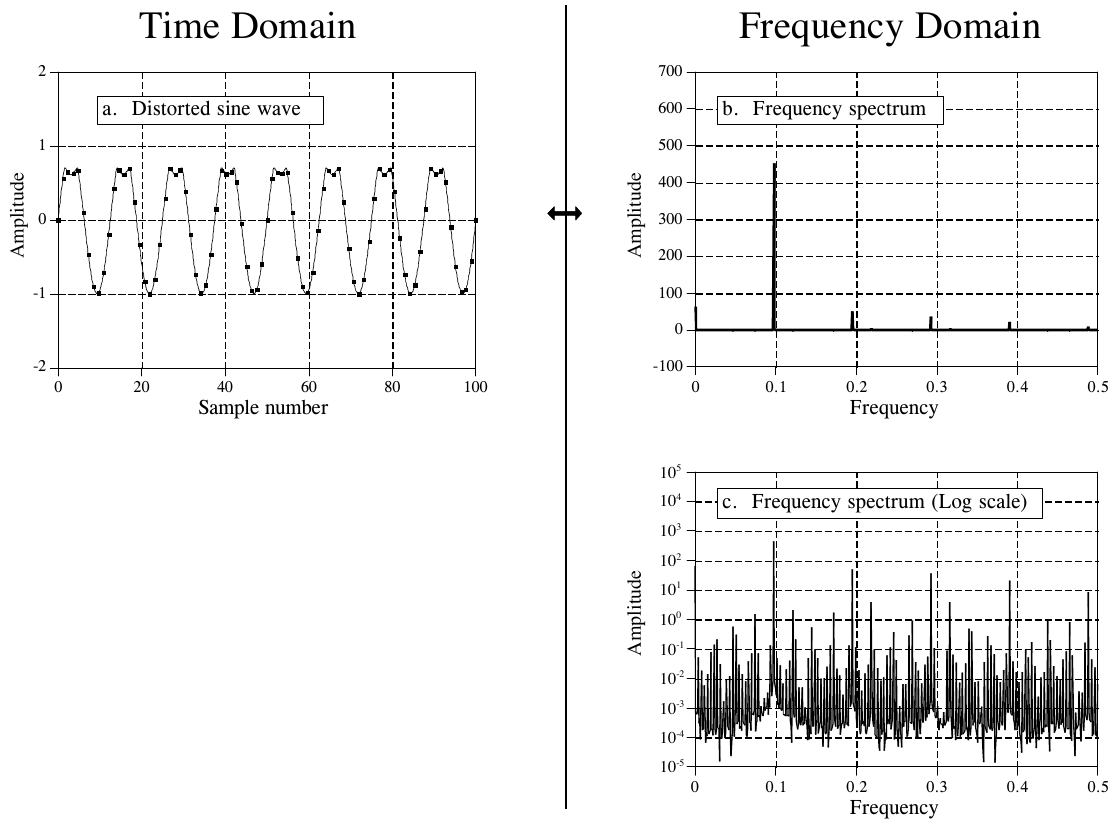
\includegraphics[width=0.929\linewidth,height=0.8\textheight,keepaspectratio]{assets/ch11/fig11-08.png}
\caption*{\textbf{图 11-8　谐波混叠。} 图 (a) 和 (b)
分别是一个失真的正弦波及其频谱。频率高于 0.5 的谐波会混叠到 0 和 0.5
之间的某个频率。图 (c)
用对数刻度画出同一频谱，显示出许多幅度很低的混叠峰。 （Time Domain =
时域，Frequency Domain = 频域；a. Distorted sine wave = 失真的正弦波；b.
Frequency spectrum = 频谱；c.~Frequency spectrum (Log scale) =
频谱（对数刻度）。Amplitude = 幅度，Sample number = 采样序号，Frequency
= 频率。原书图注说明排在左下方，裁图时已去掉，译文见上。）}
\end{figure}

要明白，这个例子是在信号已经数字化表示之后才使它失真的。如果这种失真发生在模拟信号中，你会在数字化之前用抗混叠滤波器(antialias
filter)去掉这些惹麻烦的谐波。只有直接对离散信号做非线性运算时，谐波混叠才是个问题。即便如此，这些混叠谐波的幅度也常常低到可以忽略。

谐波的概念还有另一个用处：它解释了为什么 DFT
把时域和频域都看作周期性的。在频域中，N 点 DFT 由 N/2+1
个等间距的频率组成。你可以把这些采样之间的频率看作 (1) 值为零，或者 (2)
不存在。不管哪种看法，它们都不参与时域信号的合成。换句话说，离散频谱由谐波组成，而不是由一段连续的频率范围组成。这就要求时域以频域中最低的正弦信号的频率（即基频）呈周期性。不计直流值，频域中表示的最低频率每
N 个采样完成一个完整周期，因此时域以 N
为周期呈周期性。换句话说，如果一个域是离散的，另一个域就必然是周期性的，反之亦然。这对傅里叶变换家族的四个成员都成立。由于
DFT
把两个域都看作离散的，它也必然把两个域都看作周期性的。每个域中的采样，代表的是另一个域的周期性所对应的谐波。

\section{啁啾信号}

啁啾信号(chirp
signal)是解决回声定位系统（如雷达和声呐）中一个实际问题的巧妙方法。图
11-9 是啁啾系统的频率响应。幅度恒为一，而相位是一条抛物线：

\textbf{公式 11-7}　啁啾系统的相位。

\[\mathrm{Phase}\;X[k] = \alpha k + \beta k^2\]

\begin{quote}
\textbf{译注：} 原书本章的公式编号从 11-4 直接跳到 11-7，没有 11-5 和
11-6，照原书保留。
\end{quote}

\begin{figure}[htbp]
\centering
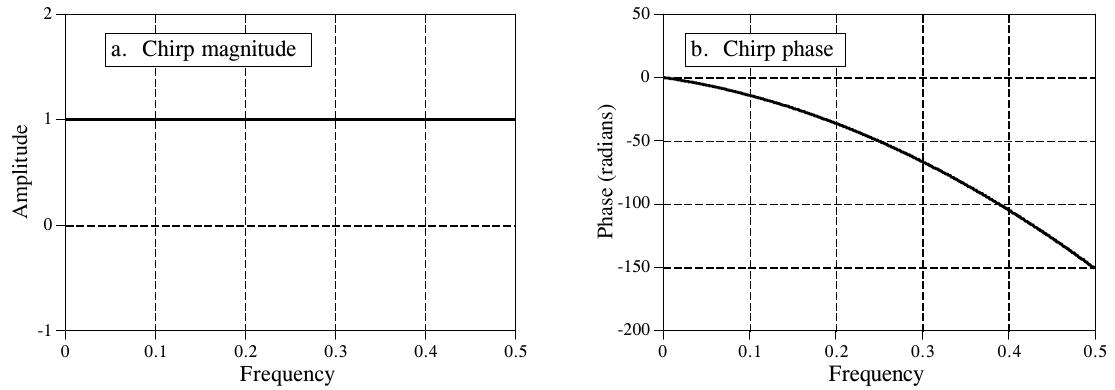
\includegraphics[width=0.929\linewidth,height=0.8\textheight,keepaspectratio]{assets/ch11/fig11-09.png}
\caption*{\textbf{图 11-9　啁啾系统的频率响应。} 幅度是常数，相位是一条抛物线。
（a. Chirp magnitude = 啁啾幅度；b. Chirp phase = 啁啾相位。Amplitude =
幅度，Phase (radians) = 相位（弧度），Frequency = 频率。）}
\end{figure}

参数 α
给相位引入一个线性斜率，也就是说，它只是按需要把冲激响应向左或向右平移。参数
β 控制相位的弯曲程度。这两个参数的选取必须使频率 0.5 处（即 k =
N/2）的相位是 2π 的整数倍。记住，只要直接修改相位，频率 0 和 0.5
处的相位都必须为零（或 2π 的整数倍，两者是一回事）。

图 11-10
展示了一个冲激进入啁啾系统，以及离开系统的冲激响应。冲激响应是一段振荡脉冲串，开始时频率低，随时间推移变成高频。它叫啁啾信号的原因很简单：用扬声器播放时，听起来像鸟的啁啾声。

\begin{figure}[htbp]
\centering
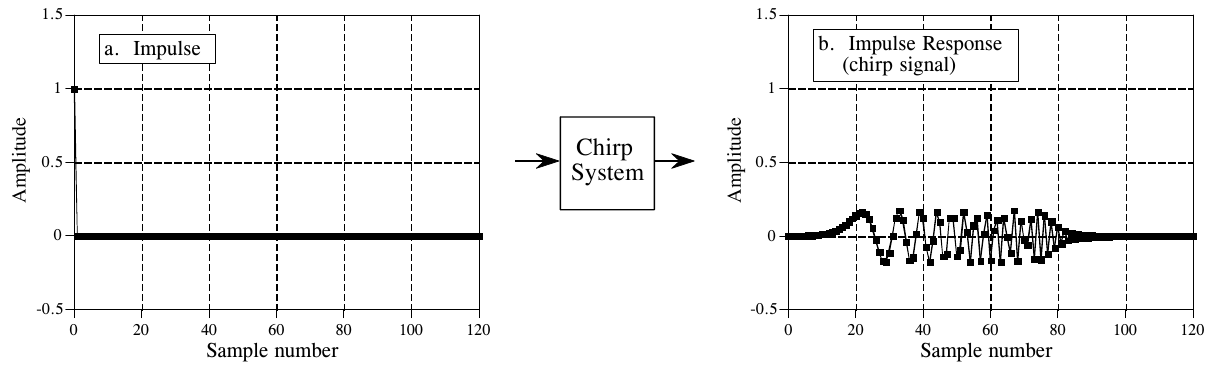
\includegraphics[width=1.000\linewidth,height=0.8\textheight,keepaspectratio]{assets/ch11/fig11-10.png}
\caption*{\textbf{图 11-10　啁啾系统。} 啁啾系统的冲激响应是一个啁啾信号。 （a.
Impulse = 冲激；b. Impulse Response (chirp signal) =
冲激响应（啁啾信号）；中间方框 Chirp System = 啁啾系统。Amplitude =
幅度，Sample number = 采样序号。）}
\end{figure}

啁啾系统的关键特点是它完全可逆。如果让啁啾信号通过一个反啁啾系统(antichirp
system)，信号又会变回一个冲激。这要求反啁啾系统的幅度为一，相位与啁啾系统相反。上一章讲过，这意味着反啁啾系统的冲激响应，可以通过把啁啾系统的冲激响应左右翻转得到。挺有意思，但它有什么用呢？

想想雷达系统是怎样工作的。一副定向天线发出一小段射频能量。飞机和其他物体把其中一部分能量反射回来，射向位于发射机旁边的无线电接收机。由于无线电波以恒定速度传播，发射信号与接收信号之间经过的时间就给出了到目标的距离。这引出了对脉冲的第一个要求：它要尽可能短。例如，1
微秒的脉冲产生的无线电波串约长 300
米。这意味着用这个系统得到的距离信息，分辨率也大约是这个长度。如果想要更好的距离分辨率，就需要更短的脉冲。

第二个要求很明显：如果想探测更远的物体，脉冲就需要更多的能量。不幸的是，更多的能量和更短的脉冲是相互矛盾的要求。产生一个脉冲所需的电功率，等于脉冲能量除以脉冲长度。既要更多能量又要更短脉冲，就使电功率的承受能力成为系统的限制因素。无线电发射机的输出级能承受的功率是有限的，超过了就会烧毁。

啁啾信号提供了一种打破这个限制的方法。在冲激到达无线电发射机的末级之前，先让它通过一个啁啾系统。这样从目标飞机上反弹回来的就不是一个冲激，而是一个啁啾信号。收到啁啾回波后，让信号通过一个反啁啾系统，把它还原成一个冲激。这使得系统中测量距离的部分看到的是短脉冲，而承受功率的电路看到的是持续时间长的信号。这种波形整形(waveshaping)是现代雷达系统的一个基本组成部分。
